\documentclass{beamer}
\usetheme{boxes}
\usefonttheme{professionalfonts}
\usecolortheme{rose}
\setbeamercovered{transparent}

\hypersetup{
    breaklinks=true,		% allows hyper-references (links) exceeding a single line
    bookmarks=true,         % show bookmarks bar?
    unicode=false,          % non-Latin characters in Acrobat’s bookmarks
    pdftoolbar=true,        % show Acrobat’s toolbar?
    pdfmenubar=true,        % show Acrobat’s menu?
    pdffitwindow=false,     % window fit to page when opened
    pdfstartview={FitH},    % fits the width of the page to the window
    pdftitle={My title},    % title
    pdfauthor={HChai},     % author
    pdfsubject={Subject},   % subject of the document
    pdfcreator={Hchai},   % creator of the document
    pdfproducer={Producer}, % producer of the document
    pdfkeywords={keywords}, % list of keywords
    pdfnewwindow=true,      % links in new window
    colorlinks=false,       % false: boxed links; true: colored links
    linkcolor=red,          % color of internal links
    citecolor=white,        % color of links to bibliography
    filecolor=magenta,      % color of file links
    urlcolor=cyan            % color of external links
}
\usepackage{natbib}
\usepackage{booktabs, calc, rotating, url}
\usepackage[T1]{fontenc}
\usepackage[latin1]{inputenc}
\DeclareMathOperator{\dif}{d \!}
\newcommand{\bm}[1]{{\boldsymbol {#1}}}

\makeatletter

%%%%%%%%%%%%%%%%%%%%%%%%%%%%%% Self defined LaTeX commands.
\providecommand{\LyX}{L\kern-.1667em\lower.25em\hbox{Y}\kern-.125emX\@}

%%%%%%%%%%%%%%%%%%%%%%%%%%%%%% Textclass specific LaTeX commands.
 % this default might be overridden by plain title style
 \newcommand\makebeamertitle{\frame{\maketitle}}%
 \AtBeginDocument{
   \let\origtableofcontents=\tableofcontents
   \def\tableofcontents{\@ifnextchar[{\origtableofcontents}{\gobbletableofcontents}}
   \def\gobbletableofcontents#1{\origtableofcontents}
 }
 \long\def\newframe#1{\@newframe#1\@framestop}%
 \def\@newframe{\@ifnextchar<{\@@newframe}{\@@newframe<*>}}%
 \def\@@newframe<#1>{\@ifnextchar[{\@@@newframe<#1>}{\@@@newframe<#1>[]}}
 \def\@@@newframe<#1>[{\@ifnextchar<{\@@@@@newframe<#1>[}{\@@@@newframe<#1>[<*>][}}
 \def\@@@@@newframe<#1>[#2]{\@ifnextchar[{\@@@@newframe<#1>[#2]}{\@@@@newframe<#1>[#2][]}}
 \long\def\@@@@newframe<#1>[#2][#3]#4\@framestop#5\frameend{%
   \frame<#1>[#2][#3]{\frametitle{#4}#5}}
 \def\frameend{} % In case there is a superfluous frame end



\begin{document}
\title{Penalized Regression with Various Design Matrix Correlation Structures}


\author{Hao Chai}


\institute{Department of Statistics and Actuarial Science\\
University of Iowa}

\makebeamertitle
\frameend{}

\section{Comparison among Three Covariance Structures}

\newframe{Problem Review}
The goal is to minimize $$||\mathbf{y}-X\bm\beta||^2_2+\sum_{i=1}^p\rho(|\beta_i|;\lambda).$$
\pause
Want to compare the performance of LASSO and MCP under different correlation structures.

Set $\bm\beta=(3, 1, -1, 3, \mathbf{0})$, $n=100$, $p=500$ and signal to noise ratio $s/n = 1.5$.
There are 200 simulated data sets.

\frameend{}

\newframe{Three Correlation Structures}
\begin{enumerate}
\item[cov0:]The columns of $X$ are independent, i.e. $\mathbf{x}_i$ and $\mathbf{x}_j$ are independent if $i\neq j$.
\item[cov1:]$corr(\mathbf{x}_i,\mathbf{x}_j)=0.8^{|i-j|}$, for $i,j=1, 2, \ldots, p$.
\item[cov2:]For $i=1, 2, \ldots, p,$ $\mathbf{u}_i=\begin{cases}N(\mathbf{0},I),& \mbox{with probability 0.1};\\
0, & \mbox{with probability 0.9}.
\end{cases}$

For $i=1, 2, \ldots, p$, $\mathbf{v}_i\stackrel{i.i.d.}\sim N(\mathbf{0}, I)$.
Then for $i=1, 2, \ldots, p, $
$$\mathbf{x}_i=\mathbf{v}_i+a \cdot \sum_{j=-3}^3\mathbf{u}_{i+j},$$
with $\mathbf{u}_{-2}=\mathbf{u}_{-1}=\mathbf{u}_{0}=\mathbf{u}_{n+1}=\mathbf{u}_{n+2}=\mathbf{u}_{n+3}=\mathbf{0}$ for the brevity of notations. In this case, $a =2$.
\end{enumerate}
\frameend{}

\subsection{Selection Error Rates for LASSO and MCP}

\newframe{Selection Error Rates for LASSO and MCP}
\begin{table}[ht]
\centering
\begin{tabular}{rlll}
  \hline
 & cov0 & cov1 & cov2 \\ 
  \hline
Ltype1 & 0.029(0.028) & 0.036(0.023) & 0(0.001) \\ 
  Ltype2 & 0.249(0.195) & 0.475(0.079) & 0.684(0.111) \\ 
  LFDR & 0.717(0.197) & 0.862(0.077) & 0.048(0.144) \\ 
  LFIR & 0.002(0.002) & 0.004(0.001) & 0.005(0.001) \\ 
  Mtype1 & 0.006(0.007) & 0.003(0.005) & 0.005(0.006) \\ 
  Mtype2 & 0.324(0.186) & 0.498(0.025) & 0.469(0.139) \\ 
  MFDR & 0.386(0.276) & 0.245(0.293) & 0.383(0.296) \\ 
  MFIR & 0.003(0.001) & 0.004(0) & 0.004(0.001) \\ 
   \hline
\end{tabular}
\end{table}
The initial letter ``L" stands for LASSO and ``M" stands for MCP. ``type1", ``type2", ``FDR" and ``FIR" are type I error rate, type II error rate, the false discovery rate and the false insignificant rate respectively.
\frameend{}

\subsection{Estimation Error Rates for LASSO and MCP}
\newframe{Estimation Error Rates for LASSO and MCP}
\begin{table}[ht]
\centering
\begin{tabular}{rlll}
  \hline
 & cov0 & cov1 & cov2 \\ 
  \hline
LL1 & 5.804(2.499) & 6.233(1.965) & 5.2(0.492) \\ 
  LL2 & 2.019(0.324) & 2.097(0.28) & 3.193(0.314) \\ 
  LXL1 & 145.357(26.384) & 115.978(21.723) & 269.357(21.373) \\ 
  LXL2 & 18.646(3.318) & 14.482(2.684) & 33.954(2.797) \\ 
  ML1 & 3.291(1.031) & 3.062(0.934) & 4.494(1.602) \\ 
  ML2 & 1.56(0.308) & 1.586(0.203) & 2.23(0.644) \\ 
  MXL1 & 111.632(20.756) & 62.65(16.676) & 192.853(49.974) \\ 
  MXL2 & 14.347(2.772) & 7.822(2.064) & 24.107(6.386) \\ 
   \hline
\end{tabular}
\end{table}
The initial letter ``L" stands for LASSO and ``M" stands for MCP. $L1=||\hat{\bm\beta}-\bm\beta||_1$, $L2=||\hat{\bm\beta}-\bm\beta||_2$, $XL1=||X(\hat{\bm\beta}-\bm\beta)||_1$ and $XL2=||X(\hat{\bm\beta}-\bm\beta)||_2$.
\frameend{}




\section{Performance of Cross-Validation}
\newframe{Covariance Structure 0}
\begin{center}
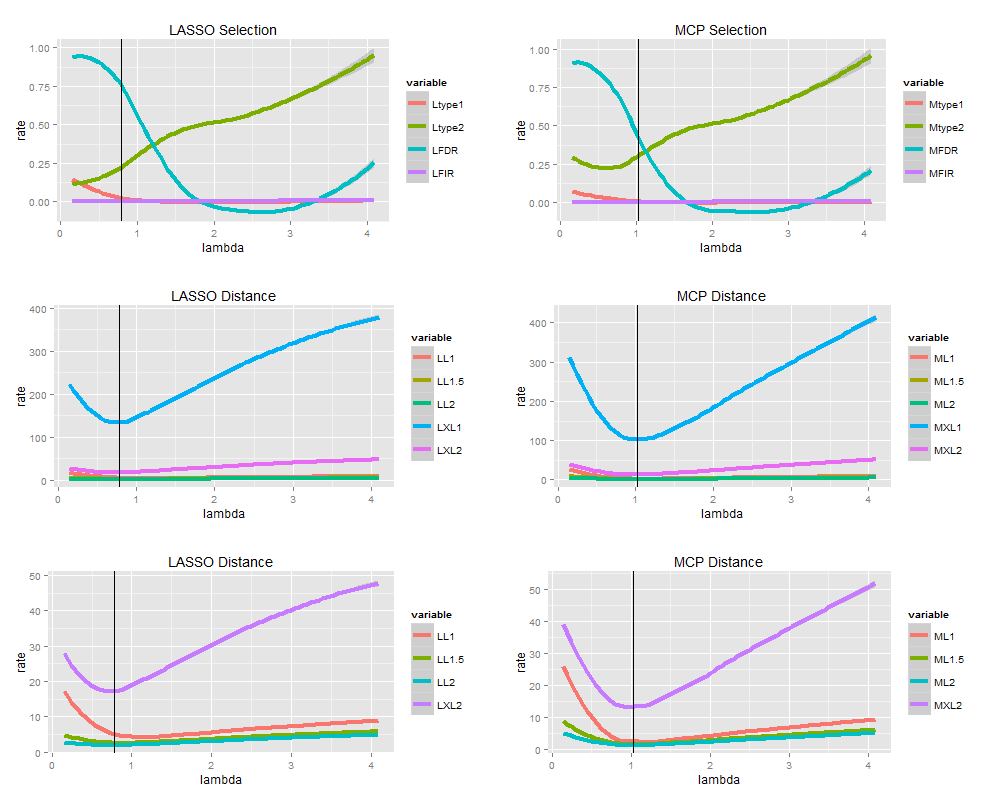
\includegraphics[width = 3.7in]{cov0.png}
\end{center}
\frameend{}

\newframe{Covariance Structure 1}
\begin{center}
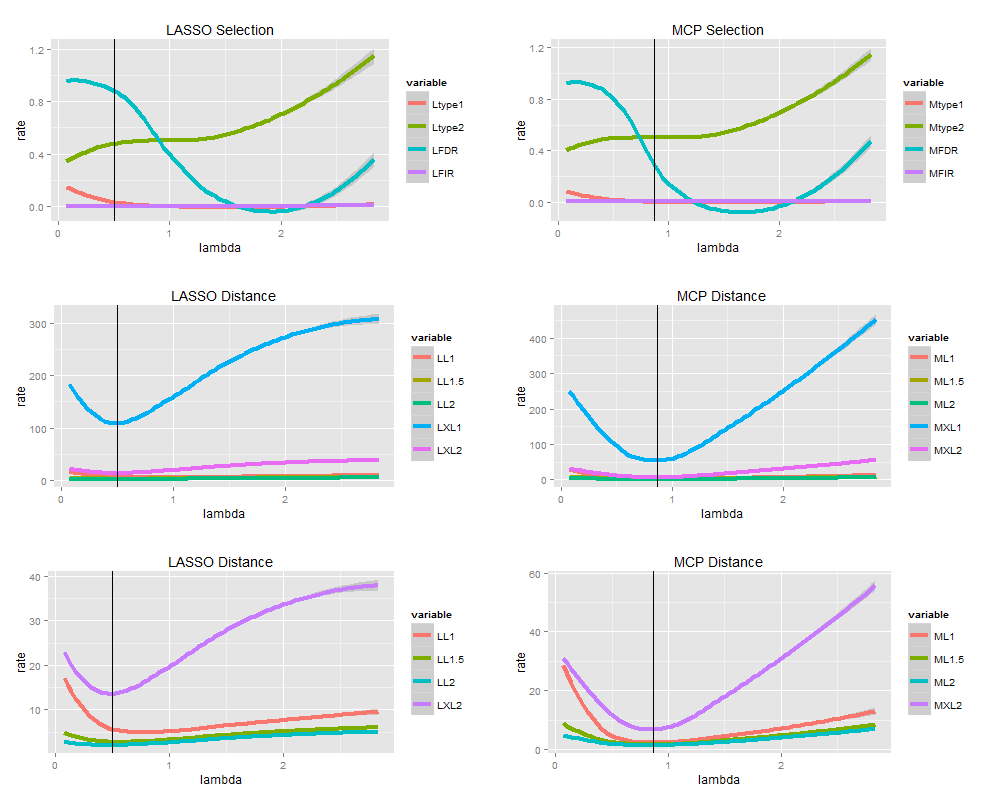
\includegraphics[width = 3.7in]{cov1.png}
\end{center}
\frameend{}

\newframe{Covariance Structure 2}
\begin{center}
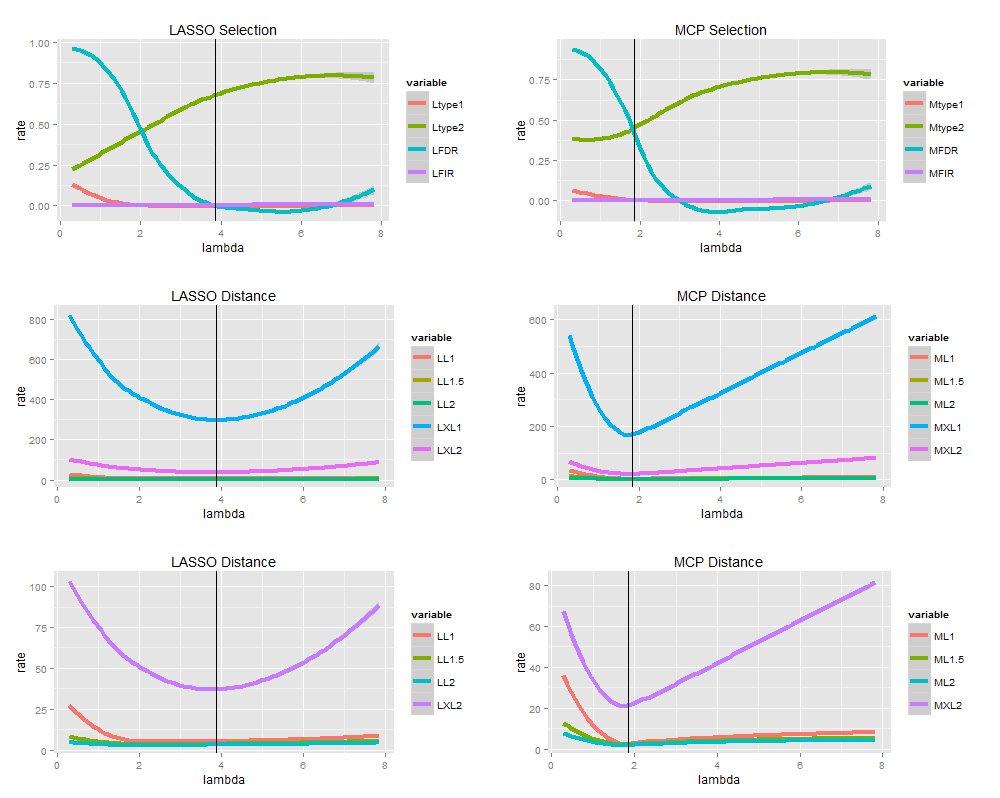
\includegraphics[width = 3.7in]{cov2.png}
\end{center}
\frameend{}

\newframe{}
Thank you!
\frameend{}



\end{document}

